\documentclass[border=8pt]{standalone}
\usepackage[utf8]{inputenc}\usepackage[T1]{fontenc}\usepackage{lmodern}\usepackage{tikz}\usetikzlibrary{arrows.meta,positioning}
\begin{document}
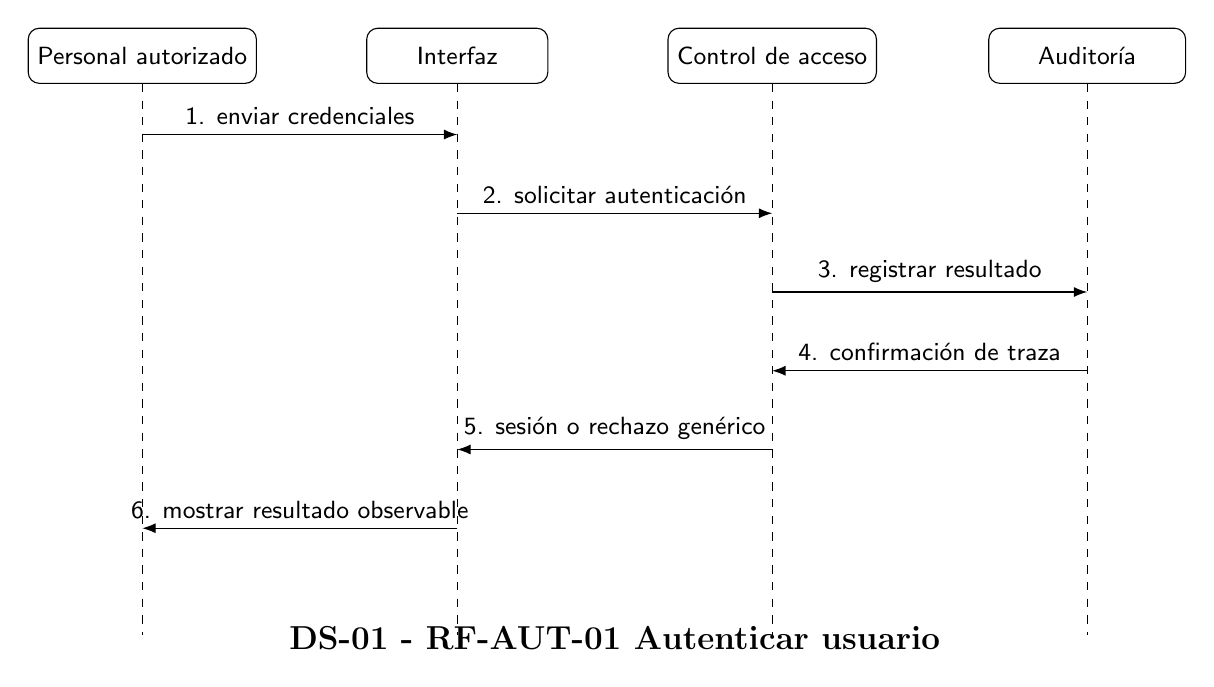
\begin{tikzpicture}[font=\sffamily\small,>=Latex]
\node[draw,rounded corners,minimum width=2.7cm,minimum height=.7cm] (actor) at (0,0) {Personal autorizado};
\node[draw,rounded corners,minimum width=2.3cm,minimum height=.7cm] (ui) at (4,0) {Interfaz};
\node[draw,rounded corners,minimum width=2.3cm,minimum height=.7cm] (auth) at (8,0) {Control de acceso};
\node[draw,rounded corners,minimum width=2.5cm,minimum height=.7cm] (audit) at (12,0) {Auditoría};
\foreach \n in {actor,ui,auth,audit}{\draw[dashed] (\n.south) -- ++(0,-7);}
\draw[->] (0,-1) -- node[above]{1. enviar credenciales} (4,-1);
\draw[->] (4,-2) -- node[above]{2. solicitar autenticación} (8,-2);
\draw[->] (8,-3) -- node[above]{3. registrar resultado} (12,-3);
\draw[->] (12,-4) -- node[above]{4. confirmación de traza} (8,-4);
\draw[->] (8,-5) -- node[above]{5. sesión o rechazo genérico} (4,-5);
\draw[->] (4,-6) -- node[above]{6. mostrar resultado observable} (0,-6);
\node[font=\bfseries\large] at (6,-7.4) {DS-01 - RF-AUT-01 Autenticar usuario};
\end{tikzpicture}
\end{document}
